In some regards, Java keeps things simple: every variable is a reference, except when it isn't.
In other regards, C keeps things simple: you always know whether the variable you're using is a value or a pointer.

\subsection{Comparing Strings}

You probably learned that when comparing Java Strings, using the equality operator \lstinline{==} is error-prone.
When comparing two String literals (or variables assigned to String literals), the equality operator usually acts as a naive programmer would expect:
\lstinline{"abc" == "abc"} evaluates to \lstinline{true}.
When one or both of the Strings are generated at runtime, such as from user input, then the equality operator rarely evaluates to \lstinline{true}:
\lstinline{userInput == "abc"} will evaluate to \lstinline{false} even when the user entered ``abc''.

The reason for this is that when comparing objects (other than boxed types), Java's comparators compare the objects' references;
that is, Java comparators compare the objects' memory addresses.
Using the \lstinline{==} operator to compare Strings evaluates to \lstinline{true} only when the two Strings occupy the same address;
that is, they are both literally the same String object.
This is why you were taught to use Java's \function{String.equals()} method to compare strings.

Comparing C strings' variables has the same pitfall:
because the string variables are pointers to the first character in their respective strings, using arithmetic comparators will compare the strings' addresses.
If you want to compare two C strings, you would use the \function{strcmp()}\footnote{See footnote~\ref{note:stringFunctions}.} function.
The wrinkle is that \function{strcmp()} returns \lstinline{0} (\textit{i.e.}, \lstinline{false}) when the two strings are equal;
you will often see the idiom \lstinline{if (!strcmp(string1, string2)) {}.

The \function{strcmp(string1, string2)} function actually performs a lexicographic comparison of the strings, returning a negative value if \lstinline{string1} occurs alphabetically earlier than \lstinline{string2}, zero if every character in the two strings match, and a positive value if \lstinline{string1} occurs alphabetically later than \lstinline{string2}.
In this regard, C's \function{strcmp()} function is more like Java's \function{String.compareTo()} method than \function{String.equals()}.

\subsection{Copying Strings}

Because Java Strings are immutable objects, you can safely copy a string by simply copying its reference (this is called \textit{aliasing}).
You can safely write the statement \lstinline{string1 = string2;} without worrying about changes to \lstinline{string2} causing changes in \lstinline{string1}
(if you were to make changes to \lstinline{string2}, it would result in a new String object being assigned to the \lstinline{string2} variable).

For mutable objects, creating an alias (that is, copying the reference) results in the situation that changes made through one variable are visible through the other variable.
For example, if you have the statements \lstinline{list1 = list2; list2.add(foo);} then \\ \lstinline{list1.size() == list2.size() && list1.contains(foo)} will evaluate to \lstinline{true}.
If the object's class implements the \lstinline{Cloneable} interface then you can make a copy of an object without aliasing it.
If you have the statements \lstinline{list1 = list2.clone(); list2.add(foo);} then \lstinline{list1.size() == list2.size()} will evaluate to \lstinline{false}.

In general, C strings are mutable.\footnote{
    The exceptions are string literals, which are immutable, and strings declared as a pointer to a constant, which if treated as mutable will result in undefined behavior.
}
This means that you generally don't want to create an alias.\footnote{
    Sometimes you can't create an alias.
    If the left-hand-side of an assignment is a constant pointer or is effectively a constant pointer -- such as an array inside a struct -- then it cannot be re-assigned.
}
Instead, use the \function{strcpy(destination, source)} or \function{strncpy(destination, source, n)}\footnote{See footnote~\ref{note:stringFunctions}.} function to copy the \lstinline{source} string into the memory pointed to by \lstinline{destination}.
The \function{strcpy()} function will continue copying until encountering the terminating \lstinline{NUL} in the \lstinline{source} string -- this is very slightly faster (not enough that you'd notice) but is safe only if you can prove that \lstinline{destination} has enough memory allocated for the string.
The \function{strncpy()} function will copy until encountering the terminating \lstinline{NUL} or until it has copied $n-1$ characters (after which it will append a terminating \lstinline{NUL}) -- this is safer because you can ensure that the string copied to \lstinline{destination} will fit within the space allocated for it.

\subsection{Allocating and Deallocating Memory}

Java's \lstinline{new} keyword allocates space for the new object, inferring the amount of space needed based on the class's definition.
In C, you use the \function{malloc()} function to allocate space\footnote{
    There are a small handful of alternate functions, each with their own use cases, but \function{malloc()} is most-suitable for this lab.
}, and you must be explicit about how much space you need.
An idiom is to combine \function{malloc()} with the \function{sizeof()} function, as you saw in PokerLab, and as you'll see near the start of Section~\ref{subsubsec:cImplementation}.

Java uses a \textit{garbage collector} to reclaim memory allocated for objects that are no longer in use.
The unpredictability of when garbage collection happens makes an automatic garbage collector unsuitable for many of C's uses.
For this reason (among others), the programmer is responsible for deallocating memory that is no longer needed.
This is done with the \function{free()} function.

While a variable will go out of scope at the end of the code block in which it was declared, memory allocated in that code block persists unless explicitly \function{free}d.
Once the last pointer pointing to that memory goes out of scope, you no longer have a way to \function{free} that memory, resulting in a \textit{memory leak}.
On the other hand, \function{free}ing memory while it is still being used by another pointer can result in undefined behavior.
This requires careful thought to make sure that you \function{free} all memory that you allocated, but only after it is safe to do so.

For many short-running programs, such as those you often write in school, you often can ignore the need to \function{free} allocated memory since all the program's memory will be reclaimed by the operating system when the program terminates.
A member of the C Standard Committee recently described this as having a maid that will clean up your mess.\footnote{
    Sarcasm alert: \url{https://twitter.com/__phantomderp/status/1619322783162568705}, \\ \url{https://twitter.com/__phantomderp/status/1619323139665846273}
}

I advise you not to rely on that ``maid'' even for a ``short-running program,'' such as this one.
In an earlier version of this lab, there were a dozen or so students whose code, when tested against a 75,000-word file, would quickly consume all the server's physical memory.
As the first of these programs thrashed the virtual memory system, it prevented other services from working effectively, including the one that I had precautionarily introduced to kill a test after a couple of minutes.
It consumed enough resources that the system administrator couldn't log in to determine why the server had slowed to a crawl.
As I was already logged in, I was able to kill the process as the system administrator was preparing to disconnect the server from the power line.
The system administrator later commented about the resources it consumed, ``You ought never to see a `T' in the memory column'' (Figure~\ref{fig:tooMuchMemoryUsed}).

\begin{figure}
    \center
    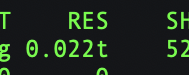
\includegraphics{too-much-memory-used}
    \caption{Screenshot showing a student's program consuming 0.022 terabytes of physical memory;
    the allocated virtual memory is not visible in the image.\label{fig:tooMuchMemoryUsed}}
\end{figure}

%\subsubsection{Idioms for Defining and Initializing \texttt{Struct} Types}
%
%In PokerLab, you worked with a struct that was defined by \lstinline{typedef} as a new type.
%In this lab, you will work with a struct defined simply as a \lstinline{struct}, without a \lstinline{typedef}.
%There are compelling arguments for and against both approaches in different use cases.
%You should learn to be comfortable with both approaches.
%
%In this lab, the function that initializes a node is also responsible for allocating space for that node.
%In PokerLab, you saw the other idiom, in which the calling function is responsible for allocating space and passing the pointer to the initializer (this pointer is analogous to Java's implicit \lstinline{this} parameter).
%The approach of having the caller allocate space seems to be more common, but both approaches are common enough to be aware of both.
%(The third idiom is not to have a separate initializing function;
%I discourage this approach.)

\subsection{Declaration vs Definition}

In C, types, variables, and functions must be \textit{declared} earlier in the file (or in an \lstinline{#include}d file) than their first use;
however, they typically do not need to be \textit{defined} until later.
A declaration provides establishes the existence and scope, and it provides enough information for the compiler to check for mismatches.
For example, a function ``prototype'' commonly found in header files simply provides the name of a function and its signature.
You can have arbitrarily many declarations for the same entity as long as they don't conflict with each other.

A definition, on the other hand, provides all the details.
(A definition is also implicitly a declaration.)
For example, a function's definition has all of its code.
An entity can only have one definition within its scope.
Functions, for example, typically have global scope, and so you cannot have multiple functions with the same name, even if they're in different files.

You are more likely, by far, to see function declarations that are not definitions than you are to see anything else declared without a definition.
In a future lab, you'll see an example of a variable declaration that has its definition in a separate file.

In this lab, we have an example of a type declaration that occurs separately from its definition.
In \textit{list.h.}, we declare a \lstinline{struct list_definition} type (and \lstinline{typedef} it to \lstinline{list_t}) without a definition.
Because none of the function prototypes in \textit{list.h} need to know anything about \lstinline{list_t} other than its existence, and because none of the code in \textit{challenge-response.c} depends on the definition, you are able to write code for the challenge-response system without regard to the underlying representation.
We provide a definition of \lstinline{struct list_definition} in \textit{array\_list.h} and another definition in \textit{linked\_list.h}.
We crafted the Makefile so that when you build \textit{arraylistlab}, only the definition in \textit{array\_list.h} is included;
similarly, when you build \textit{linkedlistlab}, only the definition in \textit{linked\_list.h} is included.
In doing so, we ensure that each executable has only one definition of \lstinline{struct list_definition}.

Note that the code in \textit{linked\_list.c} does depend on \lstinline{struct list_definition}'s definition, but that's okay because \textit{linked\_list.c} \lstinline{#include}s \textit{linked\_list.h}.


\subsection{The \lstinline{static} Keyword \\ \footnotesize{does not mean what you think it means}}

In Java, the \lstinline{static} keyword is used to make a field or method be shared among all instances of a class, and even be available without having an instance of the class.
The C programming language doesn't have classes, so clearly \lstinline{static} cannot mean the same thing.

In C, \lstinline{static} can be used in two different ways.
In a future lab, we'll see the use of \lstinline{static} for function-scoped variables.
In this lab, we have two functions in \textit{linked\_list.c} that are modified with the \lstinline{static} keyword.

When function or variable that is declared outside of any function is modified with the \lstinline{static} keyword, it no longer has global scope;
instead, its scope is limited to the file.
You can think of it as roughly corresponding to Java's \lstinline{private} visibility modifier.
This has two implications:
\begin{itemize}
    \item A file-scoped function or variable cannot be accessed from code in another file
    \item Another file-scoped function or variable of the same name can be defined in another file without violating the rule against multiple definitions
\end{itemize}
